\documentclass[11pt]{article}
\usepackage{geometry}
\geometry{a4paper, left=20mm, top=20mm}
\usepackage{amsmath}
\usepackage{graphicx}
\usepackage{hyperref}
\usepackage[T1]{fontenc}
\usepackage{polski}
\usepackage[utf8]{inputenc}

\usepackage{xcolor}

\title{Grafika Komputerowa Wirtualna Kamera}
\author{Mikołaj Kubik}

\begin{document}
\maketitle
\section{Wstęp}
Celem projektu była implementacja wirtualnej kamery, pozwalającej na 
obserwację trójwymiarowych obiektów. Kamera posiada możliwość poruszania się 
i obracania w trzech osiach oraz zmiany przybliżenia. Kod źródłowy programu oraz plik jar znajdują się w repozytorium \href{https://github.com/MikolajKubek/swing-virtual-camera}{\color{blue}GitHub}.
\section{Zmiany względem wstępnego planu}
Względem pierwotnego planu zmieniła się technologia - wykorzystałem
język java i bibliotekę swing zamiast c++ z sfml, ponieważ okazało się, 
że różnica wydajnościowa między tymi narzędziami nie wpływa w widoczny sposób na działanie programu.
\section{Analiza zagadnienia}
Program przechowuje scenę jako listę odcinków. Aby dokonać projekcji 
sceny na perspektywę kamery z każdego punktu tworzona jest macierz, na której wykonywane są następujące operacje.
\subsection{Translacja}
Transformacja sceny odpowiadająca za pozorną zmianę położenia kamery.
\begin{equation}
    T =
    \begin{bmatrix}
        1 & 0 & 0 & X\\
        0 & 1 & 0 & Y\\
        0 & 0 & 1 & Z\\
        0 & 0 & 0 & 1
    \end{bmatrix}
    \cdot
    \begin{bmatrix}
        x\\
        y\\
        z\\
        1
    \end{bmatrix}
    =
    \begin{bmatrix}
        x + X\\
        y + Y\\
        z + Z\\
        1
    \end{bmatrix}
\end{equation}
gdzie:

X, Y, Z - wektor translacji

x, y, z - współrzędne transformowanego punktu

\subsection{Skalowanie}
Transformacja sceny odpowiadająca za przybliżanie i oddalanie. 
Zastosowanie tego równania macierzowego pozwala na niezależne skalowanie 
projekcji w płaszczyznach każdej z trzech osi, jednak aby zachować zachowanie zbliżone
do prawdziwej kamery ograniczyłem się do skalowania względem osi x i y jednocześnie.
\begin{equation}
    S =
    \begin{bmatrix}
        SX & 0 & 0 & 0\\
        0 & SY & 0 & 0\\
        0 & 0 & 1 & 0\\
        0 & 0 & 0 & 1
    \end{bmatrix}
    \cdot
    \begin{bmatrix}
        x\\
        y\\
        z\\
        1
    \end{bmatrix}
    =
    \begin{bmatrix}
        SX \cdot x\\
        SY \cdot y\\
        z\\
        1
    \end{bmatrix}
\end{equation}
gdzie:

SX, SY - współczynniki powiększenia względem osi X i Y, SZ w tym przypadku wynosi 1

x, y, z - współrzędne transformowanego punktu

\subsection{Rotacje}
Transformacje sceny odpowiadające za pozorne obracanie kamery.
\subsubsection{względem osi X}
\begin{equation}
    \begin{bmatrix}
        1 & 0 & 0 & 0\\
        0 & cos \alpha & -sin \alpha & 0\\
        0 & sin \alpha & cos \alpha & 0\\
        0 & 0 & 0 & 1
    \end{bmatrix}
    \cdot
    \begin{bmatrix}
        x\\
        y\\
        z\\
        1
    \end{bmatrix}
    =
    \begin{bmatrix}
        x\\
        cos \alpha \cdot y - sin \alpha \cdot z\\
        sin \alpha \cdot y + cos \alpha \cdot z\\
        1
    \end{bmatrix}
\end{equation}
gdzie:

$\alpha$ - rotacja kamery względem osi X

x, y, z - współrzędne transformowanego punktu

\subsubsection{względem osi Y}
\begin{equation}
    \begin{bmatrix}
        cos \beta & 0 & sin \beta & 0\\
        0 & 1 & 0 & 0\\
        -sin \beta & 0 & cos \beta & 0\\
        0 & 0 & 0 & 1
    \end{bmatrix}
    \cdot
    \begin{bmatrix}
        x\\
        y\\
        z\\
        1
    \end{bmatrix}
    =
    \begin{bmatrix}
        cos \beta \cdot x + sin \beta \cdot z\\
        y\\
        -sin \beta \cdot x + cos \beta \cdot z\\
        1
    \end{bmatrix}
\end{equation}
gdzie:

$\beta$ - rotacja kamery względem osi Y

x, y, z - współrzędne transformowanego punktu

\subsubsection{względem osi Z}
\begin{equation}
    \begin{bmatrix}
        cos \gamma & -sin \gamma & 0 & 0\\
        sin \gamma & cos \gamma & 0 & 0\\
        0 & 0 & 1 & 0\\
        0 & 0 & 0 & 1
    \end{bmatrix}
    \cdot
    \begin{bmatrix}
        x\\
        y\\
        z\\
        1
    \end{bmatrix}
    =
    \begin{bmatrix}
        cos \gamma \cdot x - sin \gamma \cdot y\\
        sin \gamma \cdot x + cos \gamma \cdot y\\
        z\\
        1
    \end{bmatrix}
\end{equation}
gdzie:

$\gamma$ - rotacja kamery względem osi X

x, y, z - współrzędne transformowanego punktu

\section{Dodatkowe obserwacje}
Po rzutowaniu trójwymiarowej sceny na dwywymiarową perspektywę kamery trzecia współrzędna 
jest różna od 1. Przez jej wartość należy przeskalować współrzędne x i y wyświetlanej 
perspektywy.
Jeżeli elementy sceny znajdują się poza polem widzenia kamery ta współrzędna skali przyjmuje wartości ujemne
co powoduje pojawianie się niechcianych "artefaktów". Aby temu zapobiec ujemna trzecia współrzędna
zamieniana jest na 1.

\begin{figure}
    \caption{Centrum sceny przed i po uwzględnieniu występowania 
    ujemnych wartości trzeciej współrzędnej wektora po transformacji}
    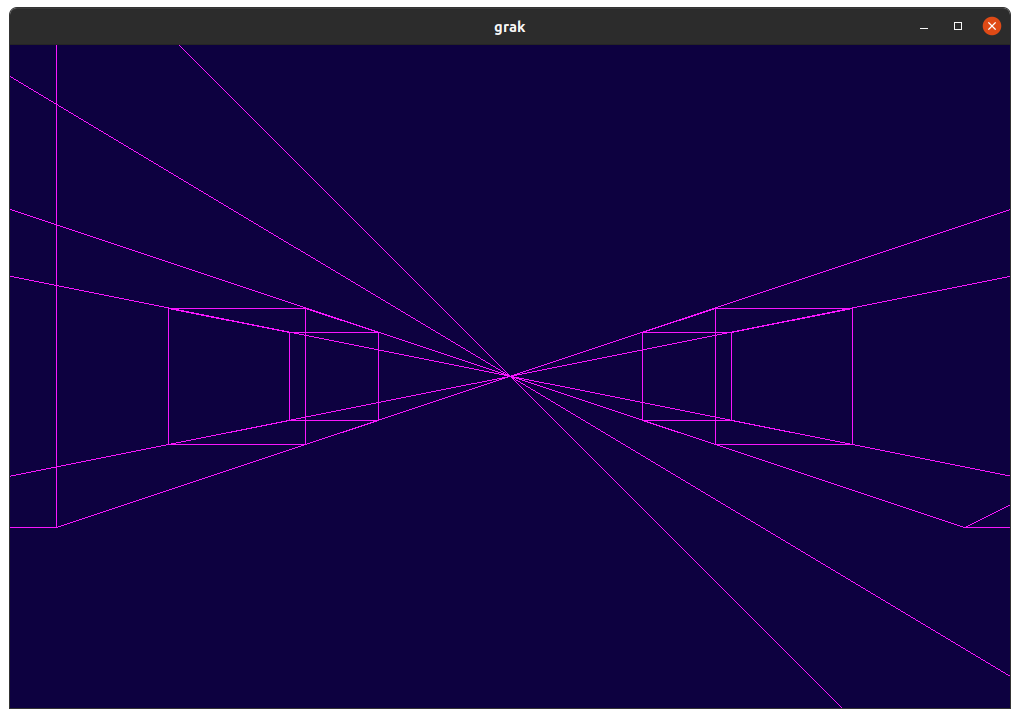
\includegraphics[width=8.5cm]{8.png}
    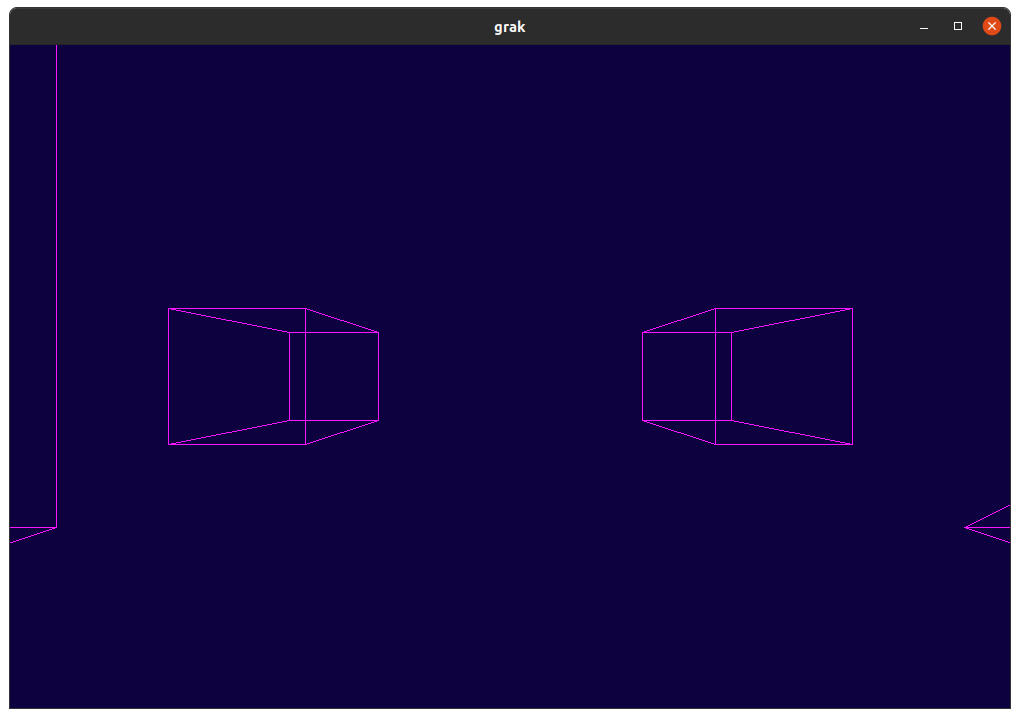
\includegraphics[width=8.5cm]{9.png}
\end{figure}
\section{Przykładowe wywołania}
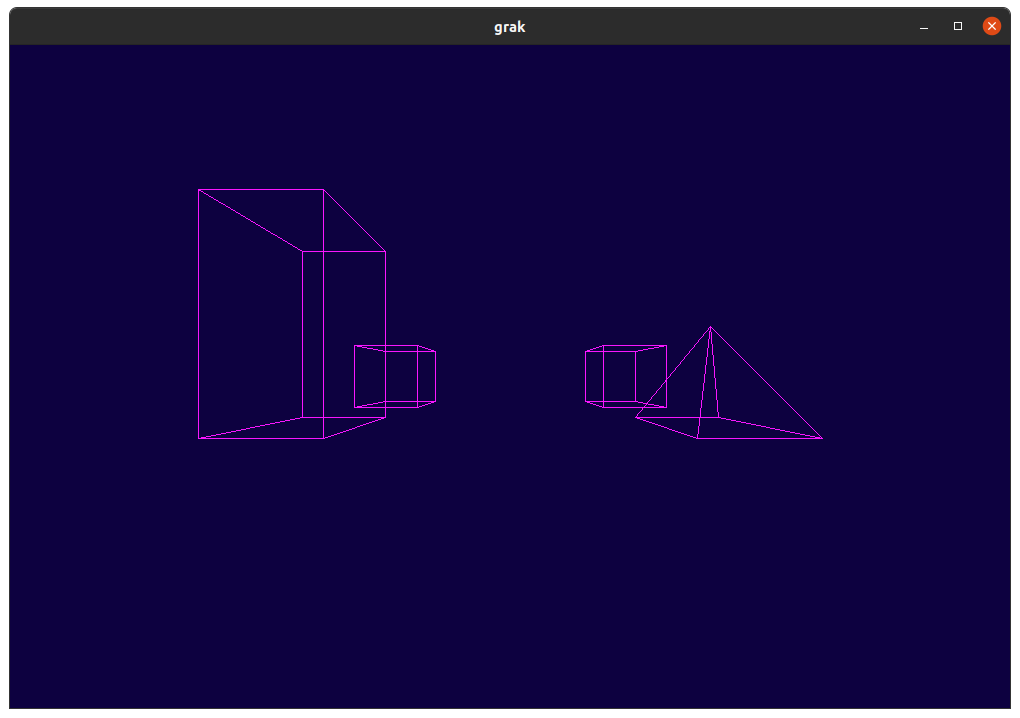
\includegraphics[width=8.5cm]{1.png}
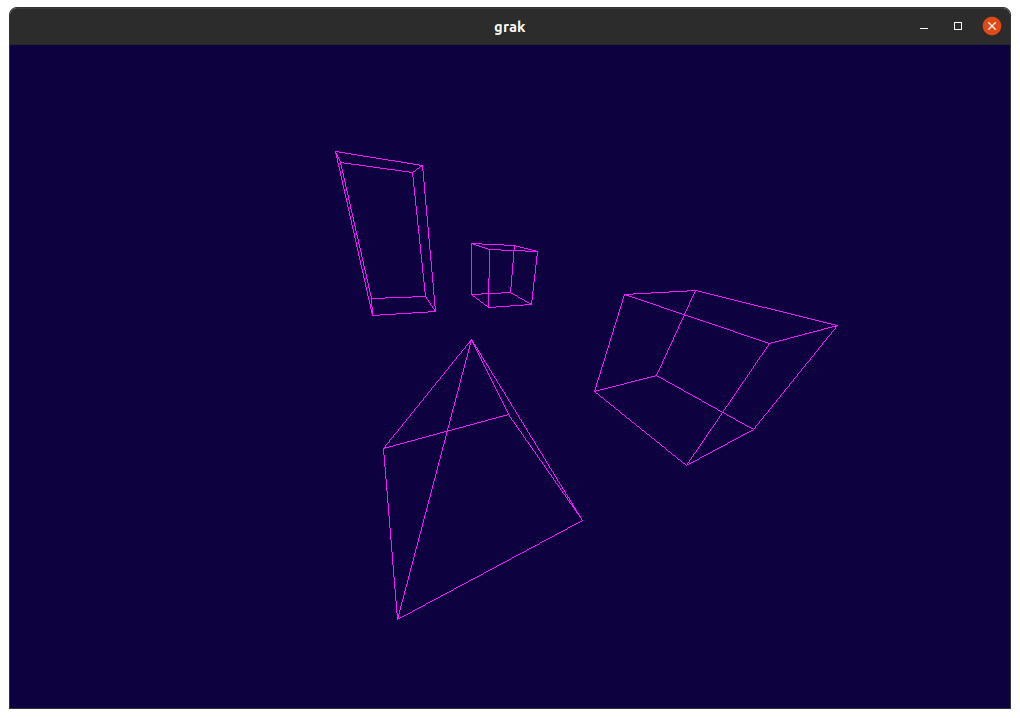
\includegraphics[width=8.5cm]{2.png}
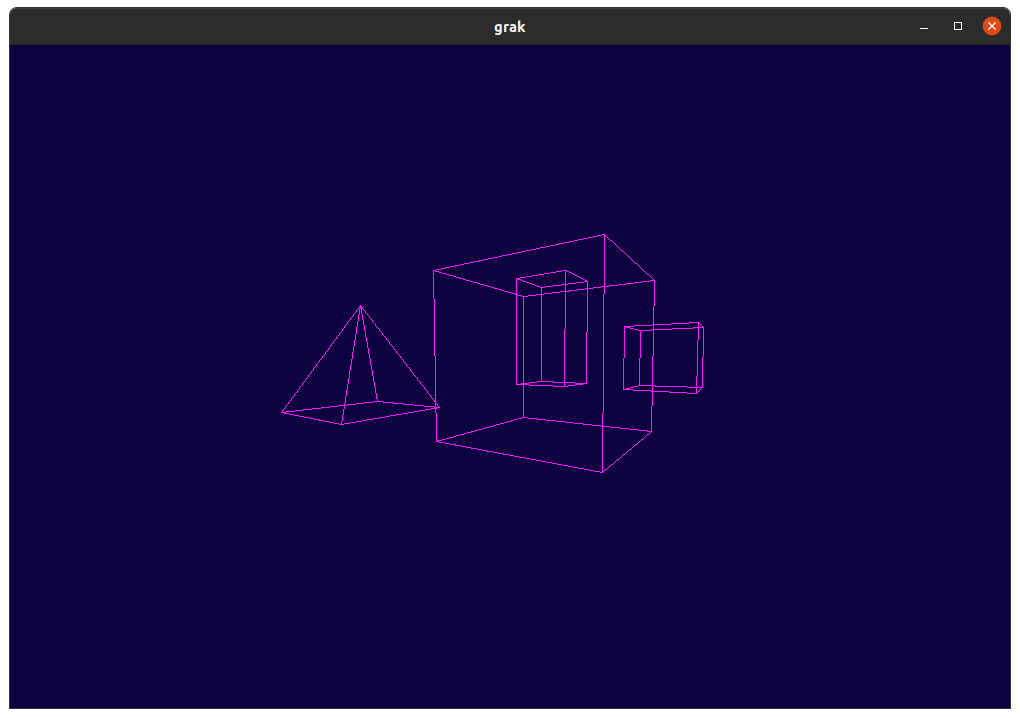
\includegraphics[width=8.5cm]{3.png}
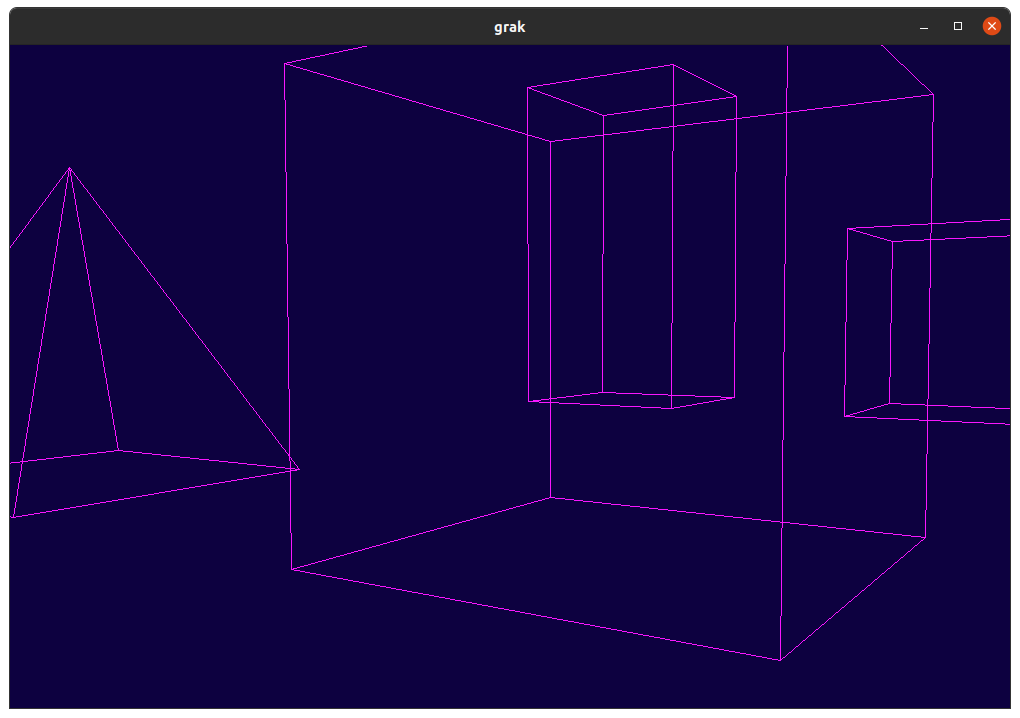
\includegraphics[width=8.5cm]{4.png}
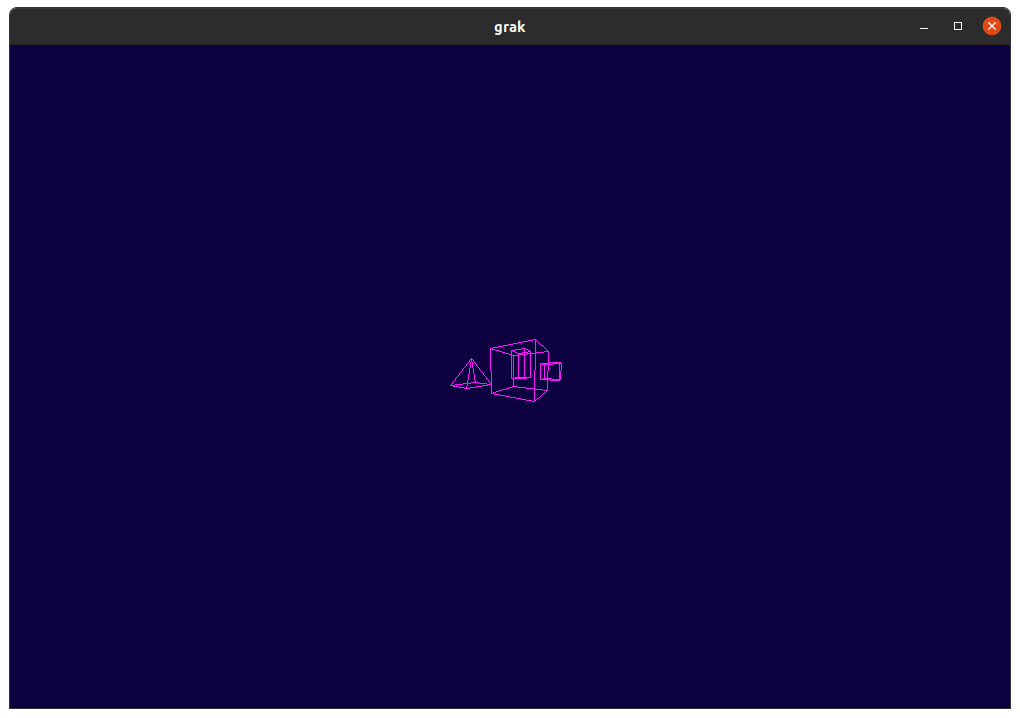
\includegraphics[width=8.5cm]{5.png}
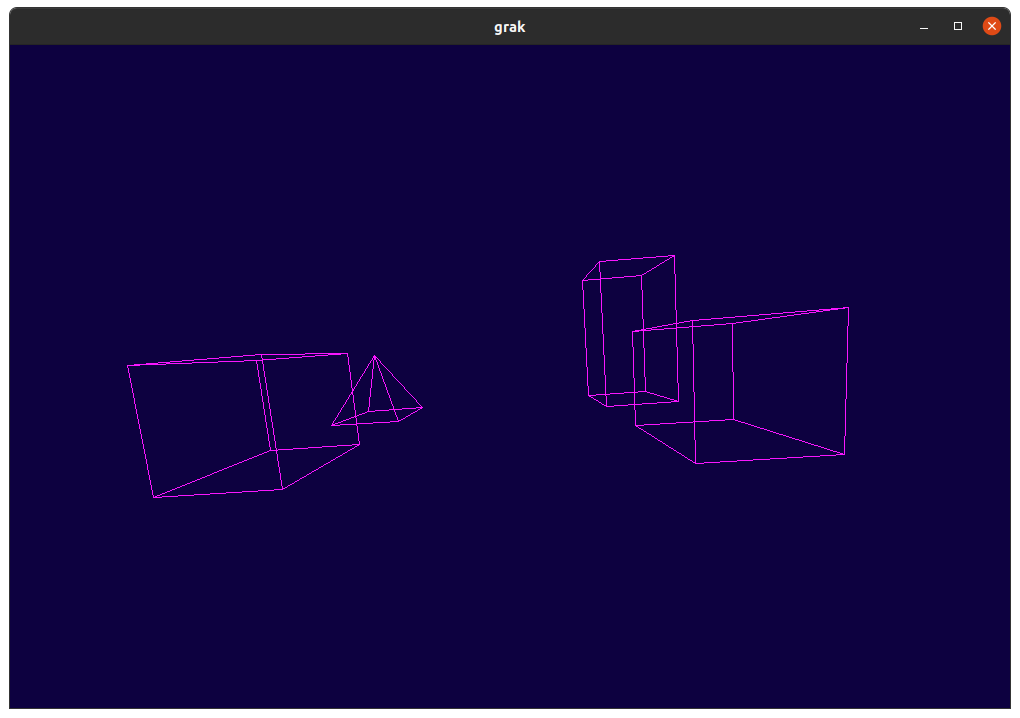
\includegraphics[width=8.5cm]{7.png}
Nagranie działania programu \href{https://youtu.be/Wztjls1sywg}{\color{blue}link}
\section{Obsługa programu}
\subsection{Wykorzystane narzędzia}
Program korzysta z javy 8 oraz The Apache Commons Mathematics Library
do obliczeń macierzowych.
\subsection{Plik wejściowy}
Opis sceny wczytywany jest z pliku zawierającego trójwymiarowe współrzędne wierzchołków, 
które program indeksuje zaczynając od zera oraz pary indeksów informujących 
które wierzchołki połączyć odcinkiem.
    \begin{verbatim}
        500 100 800
        500 100 1000
        500 -100 800
        0 1
        0 2
    \end{verbatim}
\subsection{Uruchomienie}
    \begin{verbatim}
        java -jar swing_virtual_camera.jar plik_konfiguracyjny
    \end{verbatim}
    Plik swing\_virtual\_camera.jar znajduje się w 
    out/artifacts/swing\_virtual\_camera\_jar
    względem głównego katalogu programu.
\subsection{Sterowanie}
\subsubsection{Poruszanie kamerą}
    \begin{itemize}
        \item Lewo: a
        \item Prawo: d
        \item Przód: w
        \item Tył: s
        \item Góra: space
        \item Dół: ctrl
    \end{itemize}
\subsubsection{Obracanie kamery}
    \begin{itemize}
        \item Lewo: a
        \item Prawo: d
        \item Przód: w
        \item Tył: s
        \item Pochylenie w lewo: q
        \item Pochylenie w prawo: e
    \end{itemize}
\subsubsection{Zoom}
    \begin{itemize}
        \item Powiększenie: 1
        \item Pomniejszenie: 2
    \end{itemize}
\section{Wnioski}
Praca nad projektem pokazała mi, że generowanie grafiki trójwymiarowej jest zagadnieniem złożonym 
zarówno pod kątem algorytmicznym jak i optymalizacyjnym oraz zaznajomiła mnie z podstawami
samego procesu generowania grafiki. Wykorzystanie zapisów oraz obliczeń
macierzowych znacznie ułatwia przedstawienie oraz zrozumienie i implementację problemu.
\end{document}
